% Chapter Template

\chapter{System design} % Main chapter title

\label{Chapter3} % Change X to a consecutive number; for referencing this chapter elsewhere, use \ref{ChapterX}
The given background theory of section 2 was applied for our system design. In the following we present our theoretical system and which aspects of the theory led to system design decisions. We provide a short overview in the first part, following a part where our theoretical setup is introduced. Finally we add our thoughts about algorithms that could be used.

%----------------------------------------------------------------------------------------
%	SECTION 1
%----------------------------------------------------------------------------------------

\section{Overview}
As already mentioned in the introduction, our system combines different types of data input to achieve the best position estimation. This leds to a slightly more complicated ranging process than indicated on the simplified illustration in figure \ref{fig:ranging_process}.\\
We wanted to include not only measurements from one device, but from several different data sources:
TAG and AN collect data and send it to the server, where the data is fed into the particle filter. The particle filter spreads particles accoring to TAG movement indication, restricted by the topology read from the floorplan and calculates the position likelihood according to range measurements and again the movement vector. In this phase, trilateration is already done implicitly. With respect to the likelihood, a normalized weight is assigned to each particle. The position estimation corresponds to the weighted sum of all particle positions.
An overview of the whole process is illustrated on figure \ref{fig:particle_filter_design}.

\begin{figure}[th]
\centering
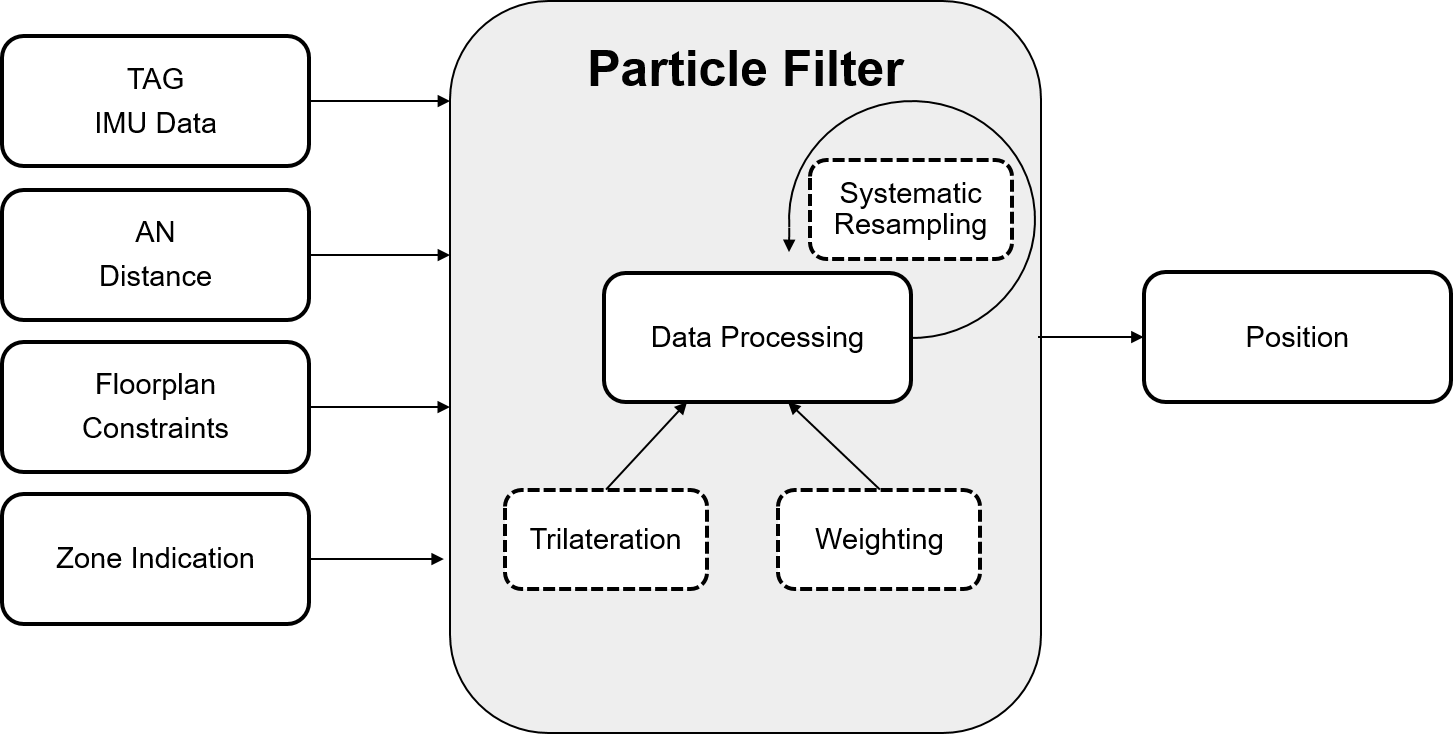
\includegraphics[width=1.0\textwidth]{Figures/particle_filter_design}
\decoRule
\caption[Particle Filter Design]{Overview of the theoretical components in our system.}
\label{fig:particle_filter_design}
\end{figure}


%----------------------------------------------------------------------------------------
%	SECTION 2
%----------------------------------------------------------------------------------------

\section{Setup}
The theoretical design on our system is shown in \ref{fig:system_design}, it works as follows:
At least three ANs, equipped with UWB technology, are placed in an indoor environment of one floor. Our algorithm runs on a seperate server, where a zoneplan and floorplan of the floor are available. A single TAG is located somewhere on the floor, it is as well equipped with UWB technology, moreover it measures acceleration and magnetic energy with the onboard IMU. The TAG continously collects data from the IMU and contemporary waits for a request from the server. The server periodically requests data via UWB from the TAG. As soon as a request is noticed at the TAG, it performs a range estimation to every AN and sends this data together with the continously collected IMU data to the server.
For every estimation period, the server has all the data needed to feed the particle filter.

\begin{figure}[th]
\centering
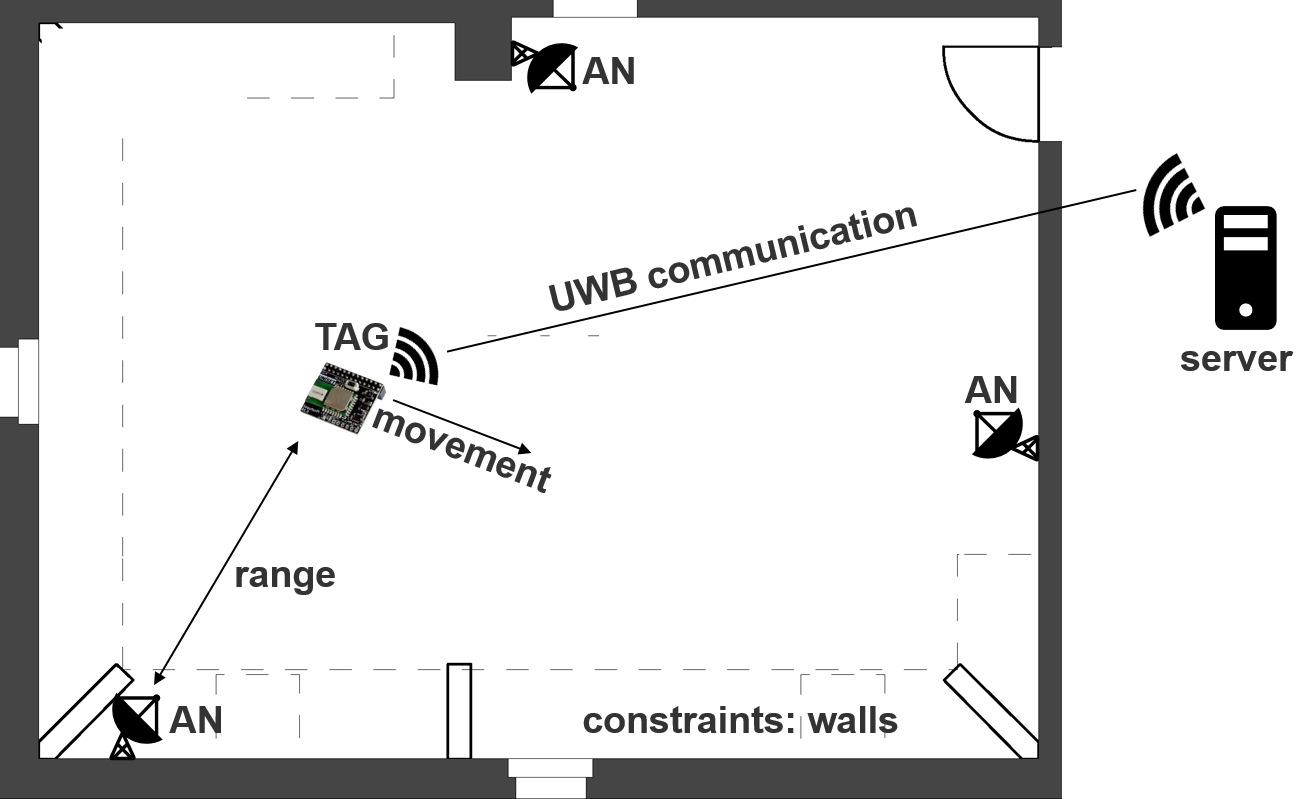
\includegraphics[width=1.0\textwidth]{Figures/system_design}
\decoRule
\caption[System Design]{Overview of the theoretical system design.}
\label{fig:system_design}
\end{figure}

%----------------------------------------------------------------------------------------
%	SECTION 3
%----------------------------------------------------------------------------------------

\section{Computations on the server}
All computations are done on the seperate server, as we would like to minimize the required computational power and energy consumption of the devices. As already mentioned, the server receives IMU data and range estimations from the nodes. This data, as well as the floorplan constrains, flow into the particle filter. These operations are done on the server:
\begin{itemize}
\item Spread the particles and validate new positions with floormap constraints
\item Evaluate UWB ranges and IMU measures to assign likelihood
\item Calculate weight function and systematically resample (and reposition) particles with low weights
\item Sum up weighted positions
\end{itemize}

In the first part, every particles is moved from its current to a new position. To validate the new position, we check if the direct trajectory between the old and the new location intersects with an impediment. If so, a new position is generated, as the last was not reachable.
The second item covers the likelihood of the new position. For every AN, the measured distance is compared to the distance from the new position to the AN. The less these two distances differ, the higher is the assigned liklihood. This is also in effect for the IMU motion, as the difference between the old and the new positon is compared to the measured IMU motion to evaluate the likelihood.
In the weighting step, every particle gets weighted by the liklihoods of the previous computations. The weights of all particles are normalized for further processing.
The last part is simply a weighted sum of the particles locations.